% =============================================================================
\section{Visibility}
% =============================================================================

In this section we will apply the model from the previous sections to the recent interferometry experiments involving a two-component \Rb{} \abbrev{bec} with two hyperfine states ${\ket{F=1,\, m_F=-1}}$ and ${\ket{F=2,\, m_F=+1}}$~\cite{Egorov2011} (the components are denoted $\ket{1}$ and $\ket{2}$ further in this section).
In the following simulations the intra- and interspecies scattering lengths for these states were taken to be $a_{11} = 100.4\,r_B$~\cite{Widera2006,Mertes2007}, $a_{12} = 98.0\,r_B$, $a_{22} = 95.44\,r_B$~\cite{Egorov2013}, and the the coefficients for the dominant loss processes are $\gamma_{111} = 5.4 \times 10^{-30} \un{cm^6/s}$~\cite{Mertes2007}, $\gamma_{12} = 1.51 \times 10^{-14}\un{cm^3/s}$, and $\gamma_{22} = 8.1 \times 10^{-14} \un{cm^3/s}$~\cite{Egorov2013}.

The experiment starts with $N = 55000$ atoms of the component $\ket{1}$ in the ground state in a cigar-shaped magnetic trap with the frequencies $f_x = f_y = 97.0\un{Hz}$ and $f_z = 11.69\un{Hz}$ in a bias magnetic field of $3.23\un{G}$, so that magnetic field dephasing is largely eliminated~\cite{Hall1998}.
The experiment is then carried out using two protocols.

\begin{figure}
    \centerline{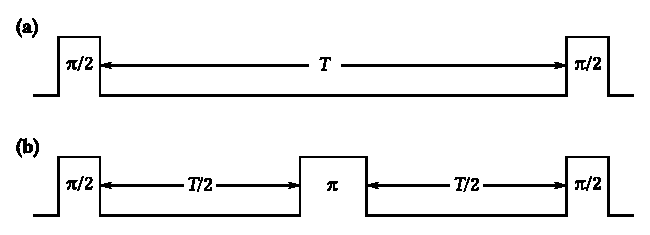
\includegraphics{figures_precreated/sequences.eps}}
    \caption{
    Timeline of the experiment for \textbf{(a)} the regular Ramsey sequence, and \textbf{(b)} the Ramsey sequence with spin echo.}
    \label{fig:bec-noise:visibility:sequences}
\end{figure}

The first protocol is the regular Ramsey sequence, depicted schematically in \figref{bec-noise:visibility:sequences},~(a): a $\pi/2$-pulse is applied by an electromagnetic coupler, creating a non-equilibrium superposition of components $\ket{1}$ and $\ket{2}$.
Mathematically, it means that coupling terms in~\eqnref{bec-noise:mean-field:cgpes-simplified} or in~\eqnref{bec-noise:wigner:single-particle-H} are enabled for a period of time equal to $t_{\mathrm{pulse}} = \theta / \Omega$, where $\theta = \pi/2$, and the Rabi frequency of the oscillator in this experiment was $\Omega = 350\un{Hz}$.
Since this pulse is short as compare to the total evolution time, it was simulated via the application of the rotation matrix~\eqnref{bec-noise:mean-field:rotation-matrix}.

During the further evolution of the system the components experience complex dynamics, separating and merging periodically~\cite{Mertes2007}.
This, in turn, leads to periodic dephasing and self-rephasing of the \abbrev{bec} components.
After some period of the free evolution the second $\pi/2$-pulse is applied, transforming the phase difference between the two components in the superposition into the population difference which can be imaged.
Many such experiments are performed with different free evolution times, contributing one time-point each, because the imaging effectively destroys the \abbrev{bec}.
A more detailed description of the experiment can be found in~\cite{Egorov2011} and in M.~Egorov's PhD thesis~\cite{Egorov2012}.

The simulations in this and the following sections used the plane wave basis (see \appref{bases} for details) and a $64\times8\times8$ spatial grid.
The integration was performed using a low-dissipation 4th-order Runge-Kutta algorithm (see \appref{numerical} for details).

The rephasing cycles can be represented by a common interferometric quantity --- the fringe contrast, or visibility:
\begin{eqn}
\label{eqn:bec-noise:visibility:visibility}
    \mathcal{V}
    = \frac{2 \left| \int \langle \Psiop_1^\dagger \Psiop_2 \rangle \upd \xvec \right|}%
        {\int \langle \Psiop_1^\dagger \Psiop_1 + \Psiop_2^\dagger \Psiop_2 \rangle \upd \xvec},
\end{eqn}
where the denominator is just the total number of atoms in the system.
This quantity can be shown to be the envelope curve of the population fringes produced by the second $\pi/2$-pulse in the experiment.
In the mean-field model the required correlations are calculated simply as
\begin{eqn}
    \tilde{n}
    & = \langle \Psiop_1^\dagger \Psiop_2 \rangle \approx \Psi_1^* \Psi_2, \\
    n_j
    & = \langle \Psiop_j^\dagger \Psiop_j \rangle \approx \Psi_j^* \Psi_j.
\end{eqn}
In the Wigner representation we have to make the correlations symmetrically-ordered first, and then~\eqnref{wigner-bec:fpe-bec:moments} gives us
\begin{eqn}
    \tilde{n}
    & = \langle \Psiop_1^\dagger \Psiop_2 \rangle
    = \langle \symprod{ \Psiop_1^\dagger \Psiop_2 } \rangle
    \approx \Psi_1^* \Psi_2, \\
    n_j
    & = \langle \Psiop_j^\dagger \Psiop_j \rangle
    = \langle \symprod{ \Psiop_j^\dagger \Psiop_j }
        - \frac{\delta_{\restbasis_j}(\xvec, \xvec)}{2} \rangle
    \approx \pathavg{ \Psi_j^* \Psi_j } - \frac{M}{2V},
\end{eqn}
where we used the fact that $\delta_{\restbasis_j}(\xvec, \xvec) \equiv M / V$ in the plane wave basis, where $M$ is the number of modes (for the grid we use $M = 64 \times 8 \times 8 = 4096$), and $V$ is the volume of the simulation area.

\begin{figure}
    \centerline{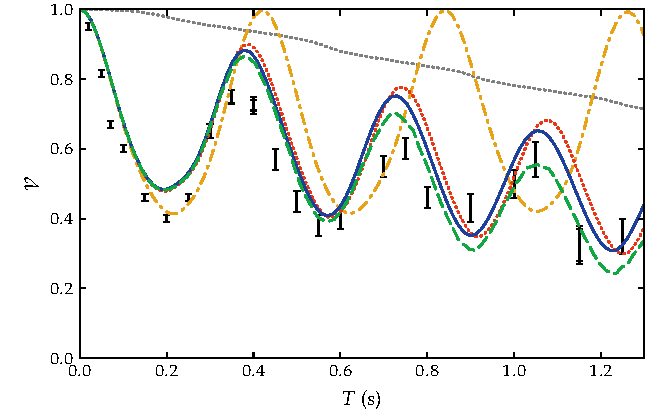
\includegraphics{figures_generated/bec_noise/ramsey_visibility_short.pdf}}

    \caption{
    Comparison of experimental and numerically simulated interferometric contrast in the regular Ramsey sequence.
    Plotted are the results obtained with mean-field and no losses (yellow dash-dotted lines), mean-field (red dotted lines), Wigner method (blue solid lines), and Wigner method with technical noises included (green dashed lines), along with the experimental points (black bars).}

    \label{fig:bec-noise:visibility:ramsey-visibility}
\end{figure}

The visibility can serve as a good example of the differences introduced by taking into account losses, quantum effects, and technical noises in the simulation of the experiment.
The inclusion of these factors in the simulation of the Ramsey sequence is demonstrated in~\figref{bec-noise:visibility:ramsey-visibility}.
The experimental results and their uncertainties are shown as the black bars in the figure.
The simplest model --- the mean-field with losses turned off --- gives results that are completely off base: the visibility is completely restored during rephasings (yellow dash-dotted lines in the figure).
The inclusion of nonlinear losses (red dotted lines) in the mean-field model closes the major part of the gap.
Application of the Wigner method (blue solid lines) has little effect on the short-time visibility (although it becomes more important at longer times, as we will se later in~\figref{bec-noise:visibility:visibility-long}).

The Wigner results can be further adjusted to account for the technical noises introduced by the experiment.

The comparison of the time dependence of the visibility obtained by the propagation of mean-field \abbrev{cgpe}s~\eqnref{bec-noise:mean-field:cgpes-simplified}, and the propagation of \abbrev{sde}s~\eqnref{bec-noise:wigner:sde} is shown in \figref{bec-noise:visibility:ramsey-visibility}.

\begin{figure}
    \centerline{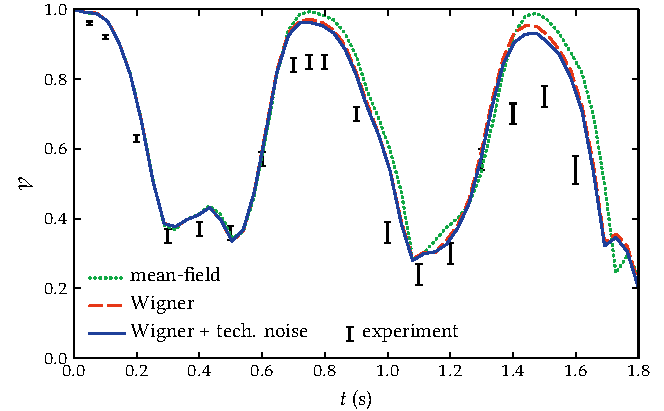
\includegraphics{figures_generated/bec_noise/echo_visibility_short.pdf}}

    \caption{
    Comparison of experimental and numerically simulated interferometric contrast in the spin-echo sequence.
    The figure shows mean-field (red dashed lines) and Wigner calculations (blue solid lines), along with the experimental points (black).
    $N = 5.5 \times 10^4$.}

    \label{fig:bec-noise:visibility:echo-visibility}
\end{figure}

\begin{figure}
    \centerline{%
    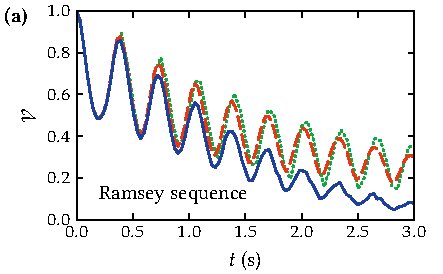
\includegraphics{figures_generated/bec_noise/ramsey_visibility_long.pdf}%
    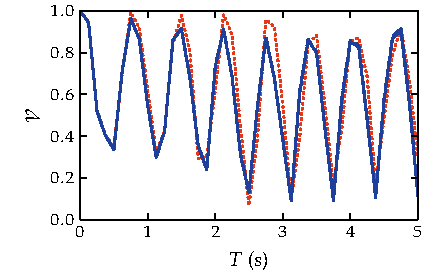
\includegraphics{figures_generated/bec_noise/echo_visibility_long.pdf}}

    \caption{
    Comparison of GPE and Wigner simulations for the normal and spin-echo sequences.
    $N = 5.5 \times 10^4$.}

    \label{fig:bec-noise:visibility:visibility-long}
\end{figure}

One of the main reasons for the inerferometry contrast decay is the assymetricity of losses.
With the populations typical for the experiment (tens of thousands of atoms or less) the two-body loss process in $\ket{2}$ is significantly stronger than the three-body one in $\ket{1}$.
This can be compensated by periodically swapping the populations of the two components by a ``spin echo'' coupler pulse of the length $\pi$.
The simplest, yet already very effective, variant is to apply the $\pi$-pulse in the middle of the evolution, as shown in~\figref{bec-noise:visibility:sequences},~(b).

The mean-field model predicts the full recover of the visibility even at very long evolution times, which is inconsistent with the experiment, as seen in~\figref{bec-noise:visibility:echo-visibility}.
On the other hand, the quasiprobability model qualitatively predicts the noticeable decay of visibility with time.
To achieve the quantitative prediction one has to include in the simulation other factors affecting the decay, namely uncertainties in the parameters of the experimental apparatus.
This can be done easily by sampling these for each of the \abbrev{sde} integration paths independently, similarly to how the initial state is sampled.

This example demonsrates that the truncated Wigner approach gives correct long-time predictions of quantum effects for the system comprised of large number of atoms.
Both of these features, large atom numbers and long time-scales, are essential to accurate interferometric measurements.
The predictions remains correct even despite multi-mode dynamical motion in three dimensions and substantial losses of most of the condensate atoms.
On longer time-scales, the experimental accuracy is limited by technical noises, and we have no data for comparisons.
